\chapter{声音：产生与传播}\label{ch:g7:sound-production}

你从小就知道，声音生于振动，
消失于真空 --- 米粒跳动，钟罩中的铃声沉寂。
你缺的只是那位信使的名字。如今你已踏入分子的世界，
声音的全程 --- 从吉他弦到你的耳膜，
穿行于空气、水或钢铁之中 ---
终于能够从内部看个清楚。

\section{信使}

\begin{definition}[介质]\label{def:g7:sound-production:medium}
称\emph{介质}\index{介质}为
声音所经过的物质，如空气、水、木材、钢铁 ---
任何状态都可以，因为它们都是分子群。声音无法穿越的，
是没有分子群的地方：真空，空荡的
舞台。
\end{definition}

\begin{proposition}[声音如何传播]\label{prop:g7:sound-production:travel}
振动的声源推动身旁的分子，分子挤向邻居，
随即弹回；邻居又推动再下一排的分子。
这一推 --- 即分子群中行进的压缩 ---
从声源向各个方向迅速扩展，
分子逐个传递，而每个分子本身只是在原位
颤动。声音是\emph{接力}，而不是奔跑者：
消息在传递，信使却始终留在原地。
\end{proposition}

\begin{omfigure}
\begin{tikzpicture}[scale=0.85]
  \draw[thick] (0.2,0.4) -- (0.2,2.2);
  \draw[thick] (0.5,0.4) -- (0.5,2.2);
  \node[above, font=\small] at (0.35,2.3) {振动的板};
  \foreach \x in {1.0,1.25,1.5,2.4,3.3,4.2,4.45,4.7,5.6,6.5,
      7.4,7.65,7.9,8.8,9.7} {
    \fill[omDef] (\x,1.3) circle (0.11);
  }
  \draw[-Stealth, very thick, omThm] (1.0,2.0) -- (2.6,2.0);
  \node[above, font=\small, omThm] at (1.8,2.1)
    {压缩正在传播};
  \node[below, font=\small] at (1.3,0.8) {稠密};
  \node[below, font=\small] at (3.3,0.8) {稀疏};
  \node[below, font=\small] at (4.6,0.8) {稠密};
  \node[below, font=\small] at (6.5,0.8) {稀疏};
  \node[below, font=\small] at (7.8,0.8) {稠密};
\end{tikzpicture}

{\small 空气中的声音：声源的推动以一连串压缩的形式传播，
即压缩的接力穿过分子群 --- 每个分子只在原地振动，
而这一图样持续向前推进。}
\end{omfigure}

\begin{example}[终于解释清楚的钟罩]\label{ex:g7:sound-production:jar}
那只著名的沉默之铃，如今道出了其中机理。抽去
空气，即抽走分子群：铃身的颤动只能推向虚空，
无从形成接力，消息也穿不过玻璃罩。
铃并未停止振动 --- 它只是失去了信使。而太空的
寂静也随之而来：星际之间没有分子群
来承载呼喊。
\end{example}

\begin{example}[响、弱与消退]\label{ex:g7:sound-production:loud}
推得越用力，压缩越强，声音就越响。随着接力
向外扩展 --- 犹如三维空间中的水波圈 --- 每次压缩
要分摊到越来越大的分子群壳层上，
因而随距离减弱：这就解释了为什么呼喊会渐远，
为什么隔壁的音乐穿过两堵墙后只剩低语。
这一切无需新的定律：分子群的物理已足以解释。
\end{example}

\begin{omfigure}
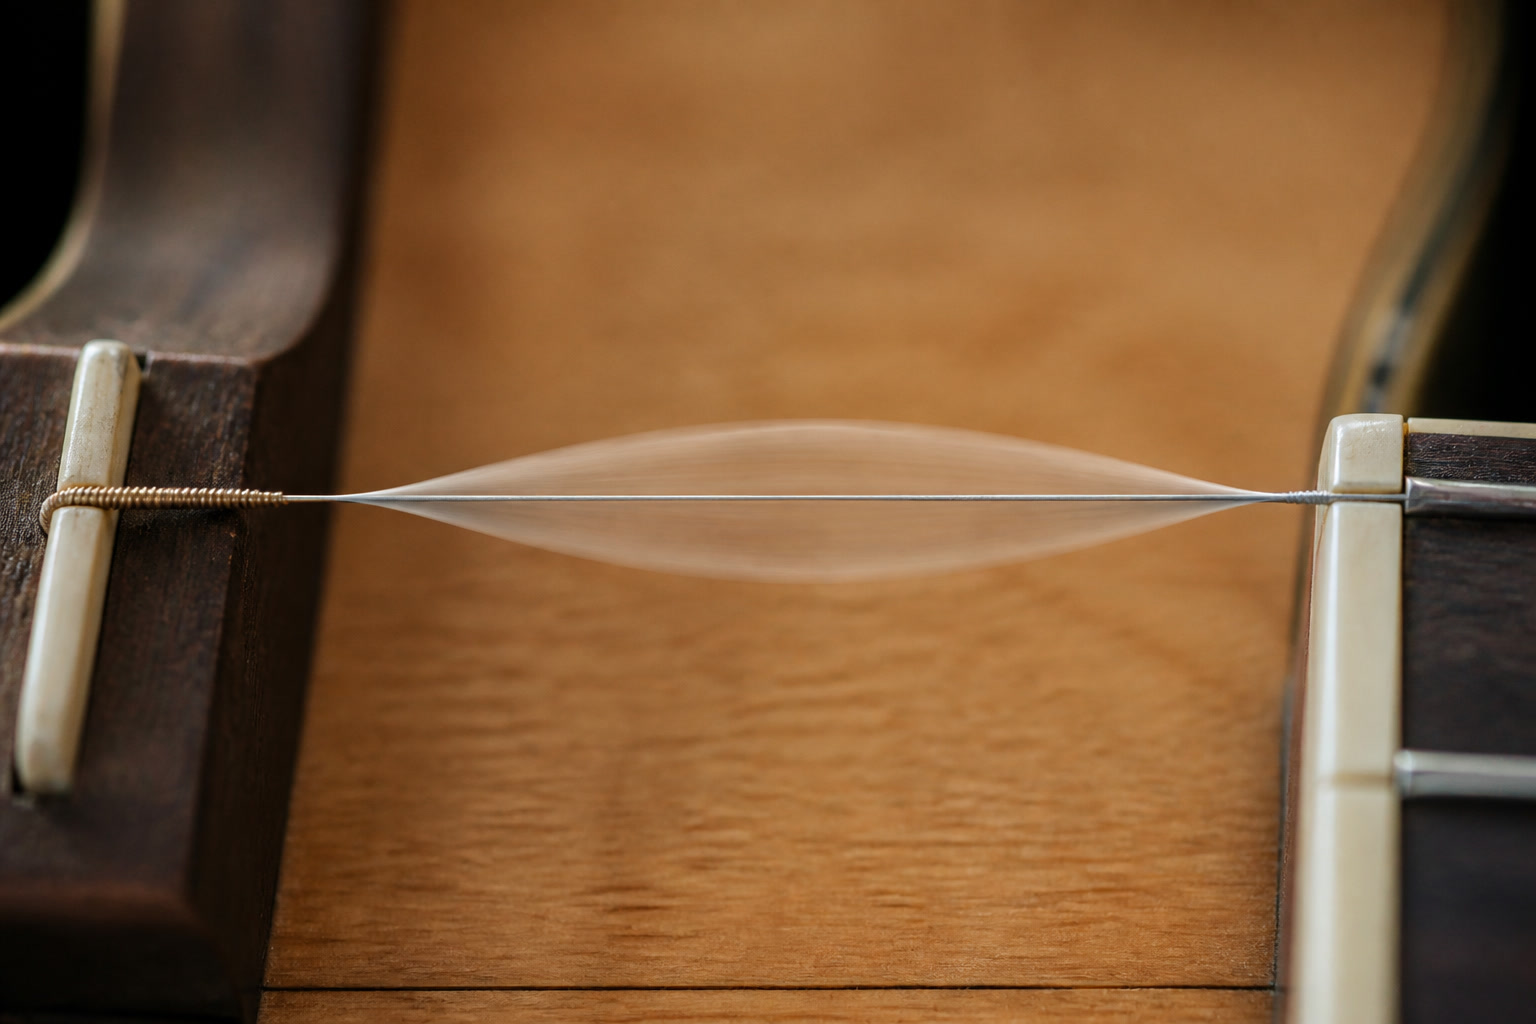
\includegraphics[width=0.55\linewidth]{images/book1/ai/g7-sound-string-blur.jpg}

{\small 琴弦鸣响时的照片：振动使其模糊成一条宽带，中央最宽，两端固定处仍然静止。}
\end{omfigure}

\section{每种介质都有自己的速度}

\begin{proposition}[声速取决于介质]\label{prop:g7:sound-production:speeds}
接力的速度是分子群的一种属性：
\begin{enumerate}
  \item 空气中：约 \qty{340}{m/s}；
  \item 水中：约 \qty{1500}{m/s} --- 快约四倍；
  \item 钢铁中：约 \qty{5000}{m/s} ---
        约为空气中的十五倍。
\end{enumerate}
规律是：介质中的分子接触越紧密，
传递推动就越快。空气中的分子飞来飞去，
必须先穿越间隙才能把推动送出；水中的分子
挨得紧密，接力迅速；钢铁中的分子排列紧固，
几乎是手递手地传递。
\end{proposition}

\begin{omfigure}
\begin{tikzpicture}
\begin{axis}[omaxis, width=10.4cm, height=4.6cm, xbar,
    xlabel={声速（\unit{m/s}）},
    symbolic y coords={air, water, steel},
    ytick=data, yticklabels={空气, 水, 钢}, xmin=0, xmax=5600,
    bar width=9pt, xtick={340,1500,5000},
    every axis plot/.append style={fill=omDef, fill opacity=0.55,
      draw=omDef}]
  \addplot coordinates {(340,air) (1500,water) (5000,steel)};
\end{axis}
\end{tikzpicture}

{\small 三群分子，三种速度：分子接触越紧，
接力就越快。}
\end{omfigure}

\begin{example}[旧场景，新数字]\label{ex:g7:sound-production:scenes}
侦察兵把耳朵贴在铁轨上：钢中的接力快于空气中的
十五倍——铁轨的警示远在隆隆声
到来之前便已抵达。鲸鱼的歌声穿越海洋：水中的接力迅速而
充沛。录音中你自己的声音听起来很陌生，
部分原因在于，说话时你听到自己的声音，既通过颅骨的
骨传导，也通过空气——两种介质，两个版本，
而只有别人才会听到仅经空气传来的那一个。
\end{example}

\section{用秒表测量声速}

\begin{method}[测量声速]\label{met:g7:sound-production:measure}
这种最古老的方法在任何运动场上仍然适用：
\begin{enumerate}
  \item 同伴站在距你 \qty{680}{m} 处（约两个
        场地长度多一点——可以步测，或利用场地的
        标线定位），手持两个锅盖；
  \item 两人在头顶上方敲击锅盖：你\emph{看到}撞击
        几乎立刻发生（光的传播可视为瞬时），并
        在看到动作的一瞬间启动秒表；
  \item 听到传来的撞击声时停止秒表：读数应非常接近
        \qty{2}{s}；
  \item 计算：$v = d/t = 680 \div 2 = \qty{340}{m/s}$。
\end{enumerate}
多次重复测量并取平均——反应时间各有波动，正如
“诚实的测量”一章所讲。数雷声就是把这一方法倒过来用：
已知 $v$，那段无声的秒数便可
算出距离。
\end{method}

\begin{example}[回声的计算]\label{ex:g7:sound-production:echo}
向悬崖拍一下手，\qty{3}{s} 后回声返回。声音
往返于悬崖之间，$d_{\text{往返路程}} = 340 \times 3 =
\qty{1020}{m}$，因此悬崖距离为其一半，即 \qty{510}{m}。每道
回声题都遵循一条规则：测得的时间对应的是
往返路程——忘记“来回”是经典错误，并
使每个答案都错误地加倍。
\end{example}

\begin{example}[认真的声呐计算]\label{ex:g7:sound-production:sonar}
测量船的声呐向下发出“咔嗒”声；海底的回声
经 \qty{0.6}{s} 返回。在\emph{水}中，$d = 1500 \times 0.6 =
\qty{900}{m}$ 为往返路程：深度 \qty{450}{m}。海豚和蝙蝠
凭本能进行同样的运算；船只则把它印在海图上。
请注意这一原则：速度由介质决定——若为水下回声
错误地代入空气中的 $340$，
便是本章的第二个经典错误。
\end{example}

\begin{remark}[“快”仍有局限]\label{rem:g7:sound-production:light}
钢中的 \qty{5000}{m/s} 听起来很了不起——直到想到光
的速度。暴风雨中，闪电的传播可视为瞬时，而
雷声三秒就跑完一千米；没有任何介质，不论是
钢，还是金刚石，都无法使声音
接近光速。光究竟有多快，以及人类
如何测出一种穿过房间只需
亿分之一秒的东西——这将是明年的故事，
将另设一章讲述。
\end{remark}

\section{练习}

\begin{exercise}[$\star$]\label{exo:g7:sound-production:1}
什么是介质？列出三种介质，以及一种
声音无法穿过的“非介质”。
\end{exercise}

\begin{exercise}[$\star$]\label{exo:g7:sound-production:2}
在接力图景中，从声源传到耳朵的是什么，
而每个分子又各自做什么？
\end{exercise}

\begin{exercise}[$\star$]\label{exo:g7:sound-production:3}
用分子观点解释玻璃罩中无声的铃铛——
以及为何电影中轰鸣的太空大战只是物理上的虚构。
\end{exercise}

\begin{exercise}[$\star$]\label{exo:g7:sound-production:4}
给出本章表格中的三种速度，并说明
介质中分子的排列与其速度之间的规律。
\end{exercise}

\begin{exercise}[$\star$]\label{exo:g7:sound-production:5}
为什么侦察兵沿铁轨传来的消息比空气中的快？
大约快了多少倍？
\end{exercise}

\begin{exercise}[$\star$]\label{exo:g7:sound-production:6}
在现场测量中，为何看到锅盖相碰的瞬间
与在声源处鸣枪起跑一样可靠？
\end{exercise}

\begin{exercise}[$\star$]\label{exo:g7:sound-production:7}
拍手声在仓库墙上的回声经 \qty{1}{s} 返回。墙
有多远？请指出会得出
\qty{340}{m} 答案的那种错误。
\end{exercise}

\begin{exercise}[$\star$]\label{exo:g7:sound-production:8}
一艘船的声呐回声经 \qty{2}{s} 返回。深度是多少？请指出
会误用 \qty{340}{m/s} 的那种错误。
\end{exercise}

\begin{exercise}[$\star\star$]\label{exo:g7:sound-production:9}
海湾上空的烟花：你看到爆炸，并在
\qty{2.5}{s} 后听到。炮弹距离有多远？为何同样的
计算无法用来判断一架\emph{喷气式飞机}的距离，
而这架飞机你能听到却看不见？
\end{exercise}

\begin{exercise}[$\star\star$]\label{exo:g7:sound-production:10}
一位一只耳朵浸在水下的游泳者，
听到池底扬声器的声音，早于站在池边的朋友通过空气听到它——
尽管朋友离扬声器更近。请结合表格解释这一现象。
\end{exercise}

\begin{exercise}[$\star\star$]\label{exo:g7:sound-production:11}
老铁路上流传着一个说法：把耳朵贴在铁轨上，你会听到火车
经过时\emph{两次}的声音。解释这两次到达的原因，并计算
距离 \qty{3}{km} 处的火车，两次声音到达的时间间隔（钢中声速 \qty{5000}{m/s}，
空气中 \qty{340}{m/s}——保留一位小数即可）。
\end{exercise}

\begin{exercise}[$\star\star\star$]\label{exo:g7:sound-production:12}
设计一个测量平静湖泊\emph{水中}声速的方案，
所用器材包括防水响板、
位于 \qty{750}{m} 外的水听器（即水下麦克风），
以及一台录音机。该录音机旁还接有普通麦克风，
用以同时记录响板在空气中发出的拍击声。
解释如何比较两段录音中记录的两次到达时刻，
从而求出水中声速，并计算两次到达之间的预期时间差。
\end{exercise}

\section{问题：峡谷测绘}

\begin{problem}[{周末问题 --- 用耳朵测绘无声峡谷；
借助回声、铁轨与河水深度；
测量员的工具包}]\label{pb:g7:sound-production:1}
一支测量队借助秒表、一台声呐装置和本章所学的物理知识，
测绘一条偏远峡谷。声速分别为：空气中 \qty{340}{m/s}，
水中 \qty{1500}{m/s}，钢中 \qty{5000}{m/s}。

\medskip\noindent\textbf{第一部分 --- 利用回声测宽度。}
\begin{enumerate}
  \item 站在东侧崖边拍一下手，
        回声经西侧崖壁反射，在 \qty{4}{s} 后返回。
        此处峡谷的宽度是多少？
  \item 在较窄处，回声在 \qty{1.5}{s} 后返回。
        此处宽度是多少？
  \item 一名测量员站在两面平行崖壁\emph{之间}，
        拍手一次，听到两个清晰可辨的回声：分别在
        \qty{1}{s} 和 \qty{2}{s} 之后。每面崖壁距测量员多远，
        沿此直线的峡谷宽度是多少？
  \item 第一部分中最大的测量误差为何来自人手按秒表，
        而不是公式本身？（请说明重复测量的
        经验原则。）
\end{enumerate}

\medskip\noindent\textbf{第二部分 --- 下方的河流。}
\begin{enumerate}[resume]
  \item 将声呐装置浮于河面，向河底发射声波：
        回声在 \qty{0.2}{s} 后返回。河水有多深？
  \item 同一装置向水下一块巨石的方向横向发射声波，
        回声在 \qty{0.4}{s} 后返回。
        巨石距离多远？
  \item 一位队友建议省电：“在船上大喊，
        用耳朵计时河底的回声。”请给出两条物理原因，
        说明此法为何会失效，而声呐却能成功。
        （想一想两种介质的分界面，
        以及喊声经空气传到水面时需要完成什么。）
  \item 河道中段河床急剧下陷：
        预测船只漂越这一落差时，
        声呐回声的时间会如何变化。
\end{enumerate}

\medskip\noindent\textbf{第三部分 --- 废弃的矿山铁轨。}
一条废弃的直线铁轨沿峡谷谷底延伸 \qty{2}{km}，
直达矿井大门。
\begin{enumerate}[resume]
  \item 在大门处的铁轨上敲击一下：计算测量员所在位置
        两次到达的时间——一次经钢轨传来，
        一次经空气传来。
  \item 测量队听到铁轨的撞击声与空气中的爆响声，两者相隔
        这一时间差。若 \qty{2}{km} 未知，请解释如何
        \emph{仅凭时间差}测出大门的距离
        （描述推理过程；具体计算留给钻研者，
        是第三部分给好学者的附加题）。
  \item 夜间浓雾笼罩峡谷，灯火与镜子都无法使用。
        测量队的三种测量途径（空气声、水声、铁轨声）中，
        哪一种受雾的影响最小？
        请说明原因。
  \item 写出测量员的记录，用三句话概括：往返规则、
        介质决定速度的规则，以及峡谷中每次计时
        由哪一种感官（眼或耳）开始，
        为何这一开始时刻可视为“瞬时”，
        请说明理由。
\end{enumerate}
\end{problem}
